\chapter{Planar Graphs}
Ajur was so enamored by Hamiltonian cycles, he was eager to meet Rishnak and learn more about them, but Rishnak wanted to introduce a different concept: drawing graphs.

Ajur said, ``I already know how to draw graphs.''

Rishnak said, ``Wait, Ajur, there's much more to it. Listen. A planar drawing of a graph is one in which no edges cross each other (except at their endpoint vertices). By definition, a \textit{planar graph} \index{planar graph} is a graph for which there exists at least one planar drawing. And if a graph does not have any possible planar drawings, we call it a \textit{non-planar graph}.''

\begin{figure}
\begin{center}
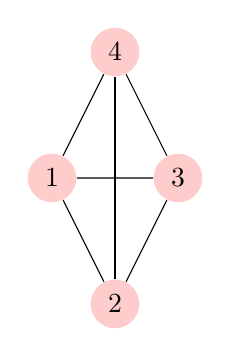
\begin{tikzpicture}
  [scale=.4,auto=left,every node/.style={circle,fill=red!20}]
  \node (n1) at (1,7) {1};
  \node (n2) at (3,3)  {2};
  \node (n3) at (5,7)  {3};
  \node (n4) at (3,11)  {4};

  \foreach \from/\to in {n1/n2,n2/n3,n2/n4,n1/n4,n3/n4,n1/n3} 
  \draw (\from) -- (\to);

\end{tikzpicture}
\caption{A drawing of complete graph~$K_4$ in which two edges cross}\label{9g1}
\end{center}
\end{figure}

In a dazzling flash of light, Rishnak waved his hands and two graphs appeared [Figure~\ref{9g1}] [Figure~\ref{9g2}]. He said, ``For example, here are two drawings of complete graph~$K_4$, the~4 in this case meaning we have four vertices. Notice that the second graph [Figure~\ref{9g2}] has no edges that cross, so we call~$K_4$ a planar graph. In other words, it displays nicely on a two-dimensional plane.''

\begin{figure}
\begin{center}
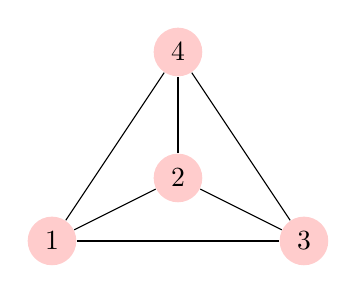
\begin{tikzpicture}
  [scale=.4,auto=left,every node/.style={circle,fill=red!20}]
  \node (n1) at (-1,7) {1};
  \node (n2) at (3,9)  {2};
  \node (n3) at (7,7)  {3};
  \node (n4) at (3,13)  {4};

  \foreach \from/\to in {n1/n2,n2/n3,n2/n4,n1/n4,n3/n4,n1/n3}
    \draw (\from) -- (\to);

\end{tikzpicture}
\caption{A planar drawing of~$K_4$ in which no edges cross}\label{9g2}
\end{center}
\end{figure}

\begin{figure}
\begin{center}
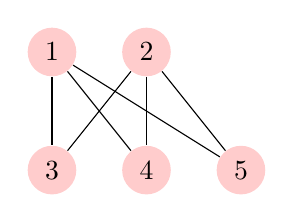
\begin{tikzpicture}
  [scale=.3,auto=left,every node/.style={circle,fill=red!20}]
  \node (n1) at (1,7) {1};
  \node (n2) at (5,7)  {2};
  \node (n3) at (1,2)  {3};
  \node (n4) at (5,2) {4};
  \node (n5) at (9,2)  {5};

   \foreach \from/\to in {n1/n3,n1/n4,n1/n5,n2/n3,n2/n4,n2/n5}
    \draw (\from) -- (\to);
    \end{tikzpicture}
\caption{Bipartite graph~$K_{2,3}$ with five vertices and six edges in which four edges cross}\label{9g3}
\end{center}
\end{figure}

Rishnak asked, ``So, Ajur, can you draw this graph''---he waved his hands and a new graph appeared [Figure~\ref{9g3}]---``as a planar graph, that is, with no edges that cross?''

Ajur studied the graph and found the task to be a bit challenging. Then, he thought of moving vertex~2 down below vertex~4, thinking that would help separate the crossed edges. He picked up a stick and drew a graph in the dirt [Figure~\ref{9g4}], smiling as he realized he had solved the problem.

\begin{figure}
\begin{center}
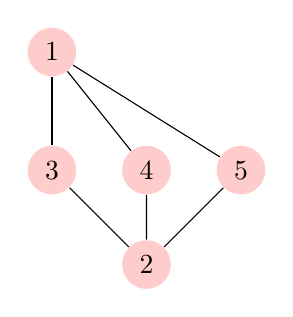
\begin{tikzpicture}
  [scale=.3,auto=left,every node/.style={circle,fill=red!20}]
  \node (n1) at (1,7) {1};
  \node (n2) at (5,-2)  {2};
  \node (n3) at (1,2)  {3};
  \node (n4) at (5,2) {4};
  \node (n5) at (9,2)  {5};

   \foreach \from/\to in {n1/n3,n1/n4,n1/n5,n2/n3,n2/n4,n2/n5}
    \draw (\from) -- (\to);
    \end{tikzpicture}
\caption{A planar drawing of bipartite graph~$K_{2,3}$ with five vertices and six edges}\label{9g4}
\end{center}
\end{figure}

Impressed, Rishnak waved his hands and another new graph appeared [Figure~\ref{9g5}]. He asked Ajur whether this new graph had a planar representation or not.

Ajur worked at this problem for some time, struggling to find a planar drawing.

At length, he said, ``I can only come up with this graph''---he pointed to the graph he had drawn [Figure~\ref{9g6}]---``but there's one edge crossing I can't get rid of.''

\begin{figure}
\begin{center}
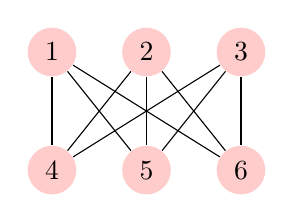
\begin{tikzpicture}
  [scale=.3,auto=left,every node/.style={circle,fill=red!20}]
  \node (n1) at (1,7) {1};
  \node (n2) at (5,7)  {2};
  \node (n3) at (9,7) {3};
  \node (n4) at (1,2)  {4};
  \node (n5) at (5,2) {5};
  \node (n6) at (9,2)  {6};

   \foreach \from/\to in {n1/n6,n1/n4,n1/n5,n2/n6,n2/n4,n2/n5,n3/n4,n3/n5,n3/n6}
    \draw (\from) -- (\to);
    \end{tikzpicture}
\caption{Bipartite graph~$K_{3,3}$ with six vertices and nine edges in which seven of the edges cross}\label{9g5}
\end{center}
\end{figure}

\begin{figure}
\begin{center}
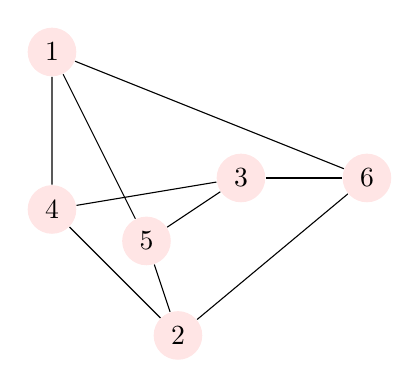
\begin{tikzpicture}
  [scale=.4,auto=left,every node/.style={circle,fill=red!10}]
  \node (n1) at (1,7) {1};
  \node (n2) at (5,-2)  {2};
  \node (n3) at (7,3) {3};
  \node (n4) at (1,2)  {4};
  \node (n5) at (4,1) {5};
  \node (n6) at (11,3)  {6};

   \foreach \from/\to in {n1/n6,n1/n4,n1/n5,n2/n6,n2/n4,n2/n5,n3/n4,n3/n5,n3/n6}
    \draw (\from) -- (\to);
    \end{tikzpicture}
\caption{A drawing of bipartite graph~$K_{3,3}$ in which just two edges edges cross}\label{9g6}
\end{center}
\end{figure}

Rishnak told Ajur that bipartite graph~$K_{3,3}$ does not have a planar representation. He said, ``There is a well-known related puzzle credited to Sam Loyd, an American recreational mathematician and puzzler. Let's say there are three houses, which we can represent as vertices~1, 2, and~3 of~$K_{3,3}$, drawn on paper. Below them are three vertices~4, 5, and~6 representing gas, water, and electricity suppliers. The aim of the puzzle is to draw lines to get each utility into every house, but---''

Ajur chimed in, ``But without crossing any of the lines.'' Ajur laughed at the puzzle, thinking that he should read up on Loyd's puzzle books the next time he visited his local library.

Rishnak cleared his throat, not entirely happy that Ajur cut him off. He said, ``If two graphs~$G$ and~$H$ are isomorphic and if~$G$ is planar, can you say that~$H$ is also planar?''

Ajur said, ``Yes, if~$H$ is isomorphic to~$G$, then each vertex of~$H$ corresponds to some vertex of~$G$. By just relabeling the vertices of~$G$ in its planar drawing, we can obtain a planar drawing of~$H$.''

Rishnak nodded and asked, ``What can we say about trees?''

Ajur thought for a moment, then said, ``That's easy. All trees have a planar representation\footnote{Ajur liked monkeys and monkeys liked trees. It follows by transitivity that Ajur liked trees.} because there are no cycles.''

Rishnak said, ``Right, trees are indeed easy to embed in a plane as there are no cycles. There are some interesting space-filling planar representations of trees, for example this one''---he waved his hands and an intricate planar drawing appeared in front of Ajur [Figure~\ref{9g7}]. \index{space filling tree}

Ajur marveled at the drawing.

Rishnak continued, ``One way to get a planar drawing of a graph is to first embed the longest cycle in a plane, then try to place the rest of the vertices so that no edges cross one another. The longest cycle will divide the plane into two regions, an inner region (inside the cycle) and an outer region (outside the cycle).''

Ajur said, ``So the edges have to go either inside or outside the longest cycle.''

Rishnak said, ``Precisely. By trying out various possibilities, backtracking as necessary, you can eventually get a planar representation of a graph---if one exists. Of course, this process is easier said than done.''

Ajur asked, ``Is there any easier way?''

Rishnak said, ``There is in fact an efficient method of placing the edges, without any backtracking, but the details are rather complicated.'' %% maybe a footnote here describing how or where to look to read more?

\begin{figure}
\begin{center}    

 \begin{tikzpicture}[decoration=H-tree, very thick]
    \draw decorate { decorate { decorate { decorate { decorate { decorate { (0,0) -- (3,0) }}}}}};
  \end{tikzpicture}
  \caption{A planar drawing of a tree, which is self-similar}\label{9g7}
  \end{center}
\end{figure}

After a few minutes of silence in which Ajur thought about how this might work, Rishnak said, ``Remember Euler?''

Ajur nodded.

Rishnak waved his hands and a new graph appeared [Figure~\ref{fig:tetra}]. He said, ``Euler discovered a remarkable relationship between planar graphs and three-dimensional solids.  This planar graph represents a tetrahedron---a pyramid.''

Ajur asked, ``How is that a pyramid? It's two-dimensional.''

Rishnak chuckled and said, ``If you imagine stretching vertex~$a3$ out toward you, you end up with a three-dimensional solid with four sides, hence the name tetrahedron.''

Ajur studied the graph and said, ``Oh, I see now.''

Rishnak continued, ``Think of each region in a planar representation as the \textit{face} of such a three-dimensional solid. Then Euler's formula relating the number of edges~$e$, the number of vertices~$n$, and the number of faces~$f$ of a planar graph is simply this.''
\index{Euler's formula}
Rishnak waved his hands and Euler's equation appeared as follows:
\begin{equation}
\label{eqn:euler}
  f-e+n=2
\end{equation}

\begin{figure}
\begin{center}
\begin{tikzpicture}
[scale=0.7]
        \grTetrahedral
    \end{tikzpicture}
\caption{Planar graph representing a tetrahedron}
\label{fig:tetra}
\end{center}
\end{figure}

Rishnak said, ``Let me explain this a bit. Each region corresponds to a cycle in the graph that surrounds that region. It also defines the external region, which is sometimes also called the infinite region. We know there are~$n-1$ edges in a tree, so if we can find that tree in the given graph, then the rest of the~$e-(n-1)$ edges will form part of a cycle. This gets tricky and we will have to explore this at some point in the future.\footnote{Rishnak and Ajur end up discussing this in Chapter~12 when they talk about spanning trees in a connected graph and how to choose one.}
%\textbf{You implicitly pick a spanning tree, which you have not yet discussed! Consider saying: it turns out, as we'll learn in Chapter ***, that there exists a ``maximal tree" of any graph.} 
Each of these cycles correspond to an internal region---in other words, an internal face---and one external face. From this, Euler's equation (\ref{eqn:euler}) follows.''

As Rishnak spoke, he drew the following equations in the air:
\begin{eqnarray}
    \label{eqn:cycles}
    \text{internal faces}&=&e-(n-1)\nonumber\\
    \text{external faces}&=&1 \nonumber \\
    \text{total faces}&=& \text{internal faces}~+~\text{external faces} \nonumber \\
    &=&e-n+2
\end{eqnarray}

Ajur studied the equations and understood, at least for a tetrahedron. He said, ``Okay, I've constructed Platonic solids with Zometool\footnote{Zometool is a commercial construction kit for making general polyhedra.}. Does this equation work for all of these?''

Rishnak smiled and said, ``Ah yes, the Platonic solids, named after Plato, the ancient Greek philosopher. And yes, Euler's equation applies to the five Platonic solids. In other words, the graph theory behind Euler's formula can be used to relate vertices, edges, and faces of the Platonic solids.''

Rishnak waved his hands and next to the graph corresponding to the tetrahedron [Figure~\ref{fig:tetra}], four more graphs appeared [Figure~\ref{fig:cube}] [Figure~\ref{fig:octa}] [Figure~\ref{fig:dod}] [Figure~\ref{fig:ico}]. He said, ``Ajur, can you write down the number of vertices~$n$, the number of edges~$e$, and the number of faces~$f$ for each of these?''

Ajur looked at each graph in turn, then systematically wrote the values in the dirt to create his table [Table~\ref{tab:platonic}].

Rishnak smiled and said, ``Good. All Platonic solids have a planar representation, as you can see in these graphs. The reason this works is that every solid fits within a sphere in such a way that no point or vertex passes through what would be the North pole. From this, one may stereographically project the graph onto the plane.''

\vspace{0.2in}
\begin{table}[ht]
    \centering
    \begin{tabular}{||c|c|c|c||}
    \hline
    Solid & n & e& f \\ [0.5ex] 
 \hline\hline
 Tetrahedron& 4 & 6 & 4 \\ 
 \hline
 Cube & 8 & 12 & 6 \\
 \hline
 Octohedron & 6 & 12& 8 \\
 \hline
 Dodecahedron & 20 & 30 & 12 \\
 \hline
 Icosahedron & 12 & 30 & 20 \\ [1ex] 
 \hline
 \end{tabular}
    \caption{Parameters of Euler's equation for the Platonic solids}
    \label{tab:platonic}
\end{table}

\begin{figure}
\begin{center}
    \begin{tikzpicture}

        \grOctahedral[RA=5,RB=1]
    \end{tikzpicture}
\caption{Planar graph representing a octahedron}\label{fig:octa}
\end{center}
\end{figure}
\begin{figure}
\begin{center}
    \begin{tikzpicture}

        \grCubicalGraph
    \end{tikzpicture}
\caption{Planar graph representing a cube}\label{fig:cube}
\end{center}
\end{figure}
\begin{figure}
\begin{center}
    \begin{tikzpicture}
    [scale=0.8]

        \grDodecahedral[form=2] 
    \end{tikzpicture}
    \caption{Planar graph representing a dodecahedron}\label{fig:dod}
\end{center}
\end{figure}
\begin{figure}
\begin{center}
    \begin{tikzpicture}

        \grIcosahedral[form=2,RA=8]
    \end{tikzpicture}
\caption{Planar graph representing a icosahedron}\label{fig:ico}
\end{center}
\end{figure}

Rishnak said, ``Notice that each edge appears in exactly two faces. If each face is a triangle---therefore a cycle of length~3---the graph is called a \textit{maximal planar graph}. From this, we can deduce~$e=\frac{3f}{2}$, or~$f=\frac{2e}{3}$. Substituting this for~$f$ in Euler's equation (\ref{eqn:euler})''---Rishnak waved his hands and equations floated in the air in front of Ajur---``we can solve for~$e$.'' \index{maximal planara graph}

\begin{eqnarray}
  \label{eqn:maxplanar}  
    \frac{2e}{3}&=&e-n+2\nonumber\\
    -\frac{e}{3} &=&-n+2\nonumber \\
    \frac{e}{3}&=&n-2 \nonumber \\
    e&=& 3n - 6
\end{eqnarray}

Rishnak paused after showing this equation (\ref{eqn:maxplanar}), giving Ajur time to think about it, then said, ``By using this equation, we can show that complete graph~$K_5$''---he flashed his hands and a new graph appeared [Figure~\ref{9g10}]---``is non-planar. This graph has five vertices and 10 edges, so~$n=5$ and~$e=10$. But from the equation, if it were planar, then the number of edges would have to be at most~$9$.''

Ajur raised his eyebrows and said, ``Aha, I see how that works. Nice!''

Rishnak asked Ajur, ``Can you use Euler's equation to show that complete bipartite graph~$K_{3,3}$ [Figure~\ref{9g5}] with its six vertices is non-planar?''

Ajur was alert and knew that a bipartite graph only has even cycle lengths. He said, ``To have the maximum number of edges, each face has to have a cycle length of~4. Therefore,~$2e=4f$ or~$f=\frac{e}{2}$.''

Ajur scribbled down equations in the dirt and said, ``Substituting for~$f$ in Euler's equation~$f=e-n+2$ (\ref{eqn:euler}), we get~$-\frac{e}{2}=n-2$, which we can write as~$e=2n-4$.''

Rishnak smiled as Ajur went on, ``Substituting~$n=6$, we get~$e=8$. That's the maximum number of edges possible, but~$K_{3,3}$ has nine edges, which is more than eight. Therefore, we have proven that~$K_{3,3}$ is non-planar!''

\begin{figure}
\begin{center}
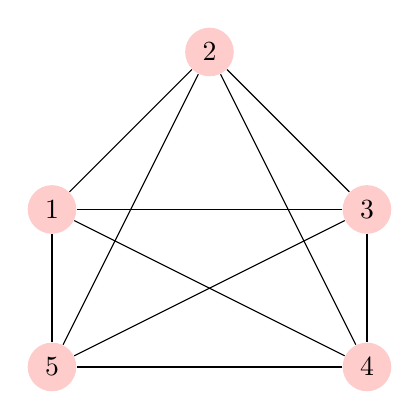
\begin{tikzpicture}
  [scale=.5,auto=left,every node/.style={circle,fill=red!20}]
  \node (n1) at (1,7) {1};
  \node (n2) at (5,11)  {2};
  \node (n3) at (9,7)  {3};
  \node (n4) at (9,3) {4};
  \node (n5) at (1,3) {5};

  \foreach \from/\to in {n1/n2,n2/n3,n3/n4,n4/n5,n1/n5,n1/n3,n1/n4,n2/n4,n2/n5,n3/n5}
    \draw (\from) -- (\to);

\end{tikzpicture}
\caption{Complete graph~$K_5$ with five vertices and 10 edges}\label{9g10}
\end{center}
\end{figure}

Rishnak's smile broadened. He said, ``Good, Ajur. And here's one more interesting fact. It turns out that any planar graph has not only a planar representation that we can draw, but also a representation in which each edge can be drawn as a straight line. Something to think about after we depart for the night.''

Ajur thought for a moment, then said, ``And every subgraph of a planar graph must also be a planar graph, right?''

Rishnak said, ``Yes, Ajur. Also, the operation of dividing an edge by introducing a new vertex of degree~2 will not change whether it is planar or non-planar. We could also do this twice to essentially add a new edge and not change whether the graph is planar or non-planar.''

Ajur frowned and said, ``I don't understand.''

Rishnak said, ``Have a look at this graph''---he waved his hands and a new graph appeared [Figure~\ref{9g9}]---``from the original tetrahedron graph [Figure~\ref{9g2}], we can divide an edge by adding a vertex or, in this case, we can add two vertices with a new edge between them. In the end, we still have a planar graph.''

Ajur studied the graph in front of him until he understood.

\begin{figure}[h]
\begin{center}
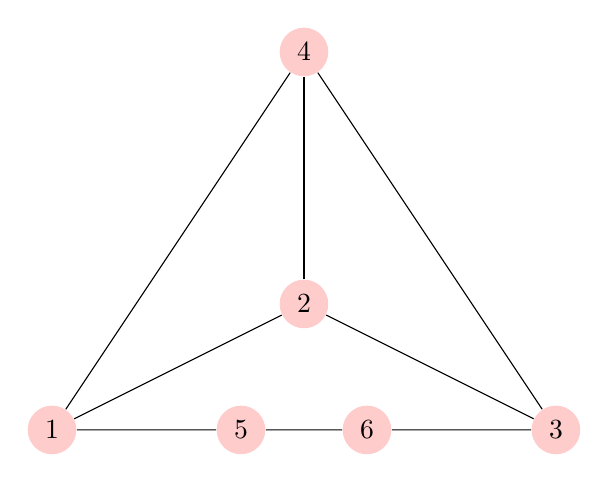
\begin{tikzpicture}
  [scale=.8,auto=left,every node/.style={circle,fill=red!20}]
  \node (n1) at (-1,7) {1};
  \node (n2) at (3,9)  {2};
  \node (n3) at (7,7)  {3};
  \node (n4) at (3,13)  {4};
  \node (n5) at (2,7) {5};
  \node (n6) at (4,7) {6};
 \foreach \from/\to in {n1/n2,n2/n3,n2/n4,n1/n4,n3/n4,n1/n5,n5/n6,n6/n3}
    \draw (\from) -- (\to);
\end{tikzpicture}
\caption{A division of original edge~$(1,3)$ by adding two new vertices (5 and~6) to the planar graph shown in Figure~\ref{9g2}}\label{9g9}
\end{center}
\end{figure}

\newpage
\subsection*{Question for the seventh day}
Rishnak stretched his arms out and said, ``We have covered a lot today. You should be ready to answer the question for the seventh day. Can you show that in a planar graph, there exists at least one vertex of degree~5?''

\textit{Before you turn the page, try to come up with an answer of your own!}

\newpage
\subsection*{Answer for the seventh day}
Ajur thought about this. He remembered Euler's equation (\ref{eqn:euler}) and said, ``Each edge occurs in exactly two faces. And the smallest face could be a cycle of length~3. Therefore, substituting~$f=\frac{2e}{3}$, we get~$\frac{2e}{3}=e-n+2$, which results in~$\frac{e}{3}=n-2$ or just~$e=3n-6$, so then\footnote{Ajur essentially derived Euler's equation (\ref{eqn:maxplanar}) once again}---''

Ajur frowned, wondering where to go with this line of thinking. At length, he said, ``This tells us that~$3n-6$ is the maximum number of edges a planar graph can have, so if all vertices have degree~6 or more, then~$e\ge3n$, contradicting that the graph is planar.''

Rishnak was happy with Ajur's answer.
Jura appeared to be getting restless, so Rishnak decided that they had had enough for that session.
They parted for the night.
